% lecture08.tex — Whitney Embedding Theorem

\section{Whitney Embedding Theorem}

So far, our $m$-manifold $M$ has been embedded in $\R^k$ where $k$ may be enormous. Can we embed it in a smaller Euclidean space?

\begin{theorem}{Strong Whitney Embedding Theorem}{strong-whitney}
    Any smooth $m$-manifold (with $m > 0$) can be embedded in $\R^{2m}$.
\end{theorem}

In this lecture, we'll only prove a weaker version where we embed it in $\R^{2m+1}$; going further down to $\R^{2m}$ requires a method known as the ``Whitney trick.''

Intuitively, it's clear why it should be possible to embed $M^m$ into $\R^{2m+1}$: since $m + m < 2m + 1$, there's enough room to wiggle things around.

\begin{center}
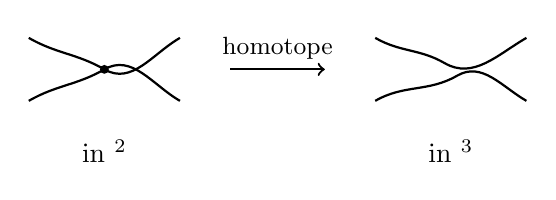
\begin{tikzpicture}[scale=0.8]
    % Self-intersecting in R^2
    \draw[thick] (-1.2,0.5) to[out=-30,in=150] (0,0) to[out=-30,in=210] (1.2,0.5);
    \draw[thick] (-1.2,-0.5) to[out=30,in=210] (0,0) to[out=30,in=150] (1.2,-0.5);
    \fill (0,0) circle (2pt);
    \node at (0,-1.3) {in $\R^2$};
    % Arrow
    \draw[->,thick] (2,0) -- (3.5,0) node[midway,above] {\small homotope};
    % Untangled in R^3
    \begin{scope}[xshift=5.5cm]
        \draw[thick] (-1.2,0.5) to[out=-30,in=150] (-0.1,0.1) to[out=-30,in=210] (1.2,0.5);
        \draw[thick] (-1.2,-0.5) to[out=30,in=210] (0.1,-0.1) to[out=30,in=150] (1.2,-0.5);
        \node at (0,-1.3) {in $\R^3$};
    \end{scope}
\end{tikzpicture}
\end{center}

\begin{remark}{}{whitney-optimal}
    Whitney's result is the best possible linear bound. In fact, when $m$ is a power of $2$, there's no embedding $\R\mathbb{P}^m \hookrightarrow \R^{2m-1}$.
\end{remark}

Now, let's prove:

\begin{theorem}{Injective Immersion in $\R^{2m+1}$}{injective-immersion}
    Every $m$-manifold admits an injective immersion in $\R^{2m+1}$.
\end{theorem}

\begin{proof}
    If $M^m \subset \R^k$, we will produce a linear projection $\R^k \to \R^{2m+1}$ that restricts to an injective immersion of $M$. Proceeding inductively, it suffices to show that: if $f \colon M \to \R^\ell$ is an injective immersion with $\ell > 2m + 1$, then there exists a unit vector $a \in \R^\ell$ such that the composition of $f$ with the projection map $\pi_a \colon \R^\ell \to H_a := \{b \in \R^\ell \mid b \perp a\}$ is still an injective immersion.

    Define maps
    \begin{align*}
        h \colon M \times M \times \R &\to \R^\ell, & (x, y, t) &\mapsto t(f(x) - f(y)), \\
        g \colon TM &\to \R^\ell, & (x, v) &\mapsto df_x(v).
    \end{align*}
    Since $\ell > 2m + 1$, by Sard, there exists a point $a \in \R^\ell \setminus \{0\}$ belonging to neither image.

    Then $\pi_a \circ f \colon M \to H_a$ is injective, since $\pi_a \circ f(x) = \pi_a \circ f(y) = ta$ implies either $t = 0$ (which means $x = y$ by injectivity of $f$) or $h(x, y, 1/t) = a$ (contradiction to our choice of $a$).

    Moreover, $\pi_a \circ f$ is an immersion, since $d(\pi_a \circ f)_x(v) = 0$ implies $\pi_a \circ df_x(v) = 0$, so $df_x(v) = ta$ for some $t \neq 0$ (by immersivity of $f$), which gives $g(x, v/t) = a$, a contradiction.
\end{proof}

For compact manifolds, injective immersions are the same as embeddings, so we have just proved the (weaker version of) embedding theorem in the compact case.

For non-compact manifolds, we need to modify the immersion to make it proper, which is a topological, not a differential problem. The fundamental technique for such generalization is the \emph{partition of unity}.

\begin{definition}{Partition of Unity}{partition-unity}
    Let $M$ be a smooth manifold. A \emph{partition of unity} $\{\rho_i\}_{i \in I}$ is a set of smooth functions $\rho_i \colon M \to \R$ such that
    \begin{enumerate}[label=(\alph*)]
        \item $\rho_i \geq 0$,
        \item each $x \in M$ has a neighborhood on which all but finitely many $\rho_i$ are identically zero,
        \item $\sum_{i \in I} \rho_i(x) = 1$ for all $x \in M$.
    \end{enumerate}

    If $\{U_\alpha\}_{\alpha \in A}$ is an open cover of $M$, then $\{\rho_i\}_{i \in I}$ is \emph{subordinate} to $\{U_\alpha\}_{\alpha \in A}$ if each $\operatorname{supp} \rho_i = \overline{\rho_i^{-1}(\R \setminus \{0\})}$ is contained in some $U_\alpha$.
\end{definition}

\begin{theorem}{Existence of Partitions of Unity}{partition-unity-existence}
    Every open cover $\{U_\alpha\}_{\alpha \in A}$ admits a countable partition of unity $\{\rho_i\}_{i \in I}$ subordinate to it.
\end{theorem}

(For now, let's take this theorem for granted.)

\begin{corollary}{Existence of Proper Functions}{proper-function}
    On any manifold $M$, there exists a proper function $f \colon M \to \R$.
\end{corollary}

\begin{proof}
    Let $\{U_\alpha\}_{\alpha \in A}$ be the set of open subsets of $M$ with compact closure. Choose a partition of unity $\{\rho_i\}_{i \in \Z_{>0}}$ subordinate to it. Define $f = \sum_{i=1}^{\infty} i\,\rho_i$. Then $f^{-1}([-j, j]) \subset \bigcup_{i=1}^{j} \operatorname{supp} \rho_i$, so $f$ is proper.
\end{proof}

Now we're ready to prove the:

\begin{theorem}{Whitney Embedding Theorem (Weak)}{whitney-weak}
    Every $m$-manifold embeds in $\R^{2m+1}$.
\end{theorem}

\begin{proof}
    Begin with an injective immersion $M \to \R^{2m+1}$. Composing with a diffeomorphism of $\R^{2m+1}$ into its unit ball, $z \mapsto \frac{z}{1 + |z|^2}$, we obtain an injective immersion $f \colon M \to \R^{2m+1}$ with $|f(x)| < 1$ for all $x \in M$.

    Let $g \colon M \to \R$ be a proper function, and define a new injective immersion
    \[
        F \colon M \to \R^{2m+2}, \qquad x \mapsto (f(x), g(x)).
    \]

    Recall that $\pi_a \circ F \colon M \to H_a \cong \R^{2m+1}$ is an injective immersion for almost every $a \in S^{2m+1}$, so pick an $a$ that is neither of the sphere's two poles.

    We claim that $\pi_a \circ F$ is proper. In fact, we will show that, for any $c$, there exists $d$ such that $(\pi_a \circ F)^{-1}(\bar{B}_c) \subset g^{-1}(\bar{B}_d)$, which is compact since $g$ is proper.

    If the claim is false, there should be a sequence of points $\{x_i\}$ in $M$ for which $|\pi_a \circ F(x_i)| < c$ but $g(x_i) \to \infty$.

    By the definition of $\pi_a$,
    \[
        w_i := \frac{1}{g(x_i)}\bigl(F(x_i) - \pi_a \circ F(x_i)\bigr) \in \R^{2m+2}
    \]
    is a multiple of $a$. As $i \to \infty$,
    \[
        w_i = \frac{F(x_i)}{g(x_i)} - \frac{\pi_a \circ F(x_i)}{g(x_i)} = \left(\frac{f(x_i)}{g(x_i)}, 1\right) - \frac{\pi_a \circ F(x_i)}{g(x_i)} \to (0, \ldots, 0, 1).
    \]
    Since each $w_i$ is a multiple of $a$, so should be the limit. This contradicts our choice of $a$, and therefore $\pi_a \circ F$ is proper.
\end{proof}
